%\section*{\lbtitle Определение химических свойств пигментов листа}
%\addcontentsline{toc}{section}{Определение химических свойств пигментов листа}

%\subsection*{Теоретические положения}

%\paragraph*{}Хлоропласты высших растений содержат в себе два типа пигментов - хлорофилл \textit{a} и \textit{b} и каротиноиды. Хлорофилл принимает в процессе фотосинтеза активное участие: под действием энергии солнечного света он передает свой электрон в элеткрон-транспортную цепь. Остальные пигменты передают энергию лишь на хлорофилл \textit{а}. 

%\paragraph*{}По химической природе \hypertarget{chlorophilus_eterus}{хлорофиллы} \textit{а} и \textit{b} – \hyperlink{hlorpophilus_etherus}{сложные эфиры} дикарбоновой кислоты хлорофиллина и двух спиртов – метанола и фитола. В центре молекулы хлорофилла расположен атом магния, соединенный с четырьмя атомами азота пиррольных колец (рисунок \ref{chlorophill}).

%\paragraph*{}Молекулу хлорофилла состоит из гидрофильного порфиринового ядра и гидрофобного хвоста из спирта фитола. 

%%%%%%%%%%%%%%%%%%%%%%%%%%%%%%%%%%%%%%%%%%%%%%%%%%%%%%%%%%%%%%%%%%%%%%%%%%%%%%%%%%%%%%%%%%%%%%%%%%%%%%%%%%% 
%\begin{figure}
%  \centering
%       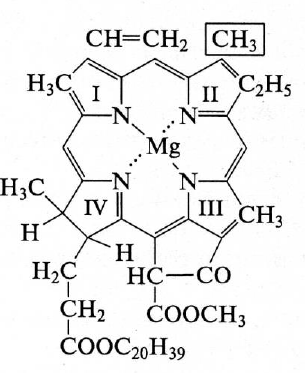
\includegraphics[width=0.3\linewidth]{pictures/chlorophill}
%\caption{Структура молекулы хлорофилла}
%\label{chlorophill}
%\end{figure}
%%%%%%%%%%%%%%%%%%%%%%%%%%%%%%%%%%%%%%%%%%%%%%%%%%%%%%%%%%%%%%%%%%%%%%%%%%%%%%%%%%%%%%%%%%%%%%%%%%%%%%%%%%%

%\paragraph*{}Фитол служит молекуле хлорофилла гидрофобным якорем, который удерживает гидрофильную порфириновую головку хлорофилла на мембране хлоропласта.

%\paragraph*{}Каротиноиды – по своей химической природе являются полиеновыми углеводородами состоящие из 40 атомов углерода и обладающие системой сопряженных двойных связей. Каротиноиды присутствуют в хлоропластах всех растений. В зеленых листьях присутствие каротиноидов скрывается хлорофиллом и они незаметны. Осенью хлорофилл в листьях разрушается, а каротиноиды остаются. За счет этого листья приобретают желтый и красный цвет.

\begin{footnotesize}

\paragraph*{}\textbf{Цель работы}: Изучить основные \hypertarget{chem_hlorophil}{химические свойства} \hyperlink{sect_hlorophilus}{пигметов листа}

\paragraph*{}\textbf{Оборудование}: Сухие или свежие листья, конические колбы с обратным холодильником, водяная баня, штатив с пробирками, пипетки на 1 мл, конические колбочки, воронки, цветные карандаши.

\paragraph*{}\textbf{Реактивы}: Этиловый спирт, бензин, 20\%-й раствор NaOH, 10\%-й раствор соляной кислоты, ацетат меди.

\end{footnotesize}

\subsection*{Ход работы}

\subsubsection*{Получение спиртовой вытяжки хлорофилла}

\paragraph*{}Измельчите ножницами приготовленные для опыта свежие листья, а затем разотрите их в ступке вместе с частицами мела и песка, постепенно подливая в ступку этиловый спирт. 

\paragraph*{}Полученную массу необходимо слить из ступки в колбу через бумажный фильтр. Закройте колбу, содержащую этот раствор пробкой и поместите на водяную баню с кипящей водой на пять минут. Полученная таким образом спиртовая вытяжка хлорофилла будет использоваться в последующих опытах.

\subsubsection*{Разделение пигментов по Краусу}

\paragraph*{}Данный метод основан на различной растворимости пигментов в спирте и бензине. Пигменты разделяются благодаря тому, что спирт и бензин не смешиваются, и находясь в одном сосуде образуют две фазы – верхнюю бензиновую и нижнюю спиртовую.

\paragraph*{}Налейте в пробирку 2-3 мл спиртовой вытяжки пигментов, приготовленной на предыдущем этапе, и добавьте к данной вытяжке 3-4 мл бензин. Затем плотно закройте пробирку пробкой и несколько раз энергично встряхните, для того чтобы жидкости, находящиеся в пробирке смешались. После этого дайте пробирке отстояться.

\paragraph*{}В результате разной растворимости пигментов, хлорофилл и каротиноиды переходят бензин, и бензин окрашивается в зелёный цвет. Ксантофилл остаётся в спиртовом слое и придаёт ему золотисто-жёлтую окраску. 

\paragraph*{}Если пигменты разделяются недостаточно чётко, добавьте в пробирку три-четыре капли воды и снова встряхните. 

\paragraph*{}Зарисуйте в отчет окраску слоёв, укажите на рисунке распределение пигментов (рисунок \ref{pigments_separation}).

\begin{figure}[h!]
\label{pigments_separation}
\caption{Схема распределения пигментов в пробирке}
	\begin{tikzpicture}
		
		\draw[rounded corners=1pt] (-0.1,4) rectangle (2.1,4.1);
		\draw (0,0) rectangle (2,4);
		\draw (0,0) rectangle (2,1);
		\draw (2,0) arc [start angle=0, end angle=-180, radius=1];
		\path[draw=red](1.5,0.5) -- (3,1);
		\path (3,1)--(5,1) node{Цвет? Пигменты?};
		\path[draw=red](1.5,-0.5) -- (3,-1);
		\path (3,-1)--(5,-1) node{Цвет? Пигменты?};

		
	\end{tikzpicture}
\end{figure}

\subsubsection*{Омыление хлорофилла щелочью}

\paragraph*{}Как было сказано \hyperlink{chlorophilus_eterus}{выше}, по своей химической природе хлорофилл является сложным эфиром. По этой причине,  при обработке хлорофилла щелочью, можно вызвать омыление эфирных групп, то есть отщепление остатков метилового спирта и фитола.

\chemfig{C_{32}H_{30}ON_{4}Mg(-[1]COOCH_{3})(-[7]COOC_{20}H_{39})} + 2NaOH $\rightarrow$ \chemfig{C_{32}H_{30}ON_{4}Mg(-[1]COONa)(-[7]COONa)} +  CH$_{3}$OH + C$_{20}$H$_{39}$OH


\paragraph*{}В результате омыление образуется соль хлорофилловой кислоты, которая сохраняет зеленую окраску хлорофилла, но при этом приобретает гигрофильные свойства в следствии  отсутствия фитольного хвоста.  

\paragraph*{}Для проведения опыта в пробирку с 2-3 мл ранее полученной вытяжки хлорофилла прилейте 1 мл 20\%-го раствора NaOH.

\paragraph*{}Взболтайте полученную смесь и на несколько минут поместите ее на водяную баню.

\paragraph*{}После вскипания смеси, снимите пробирку с водяной бани и охладите, опустив низ пробирки в ёмкость с холодной водой. К охлаждённому раствору прилейте равный объем бензина и резко встряхните пробирку. В результате каротин и ксантофилл переходят в бензиновый слой, а натриевая соль хлорофилловой кислоты остаётся в спиртовом растворе.

\paragraph*{}Зарисуйте окраску слоёв в отчет и укажите распределение пигментов.

\subsubsection*{Получение феофитина и обратное замещение водорода атомом металла}

\paragraph*{}Атом магния сравнительно слабо удерживается внутри порфиринового кольца и, при условии мягкого воздействия, под действием кислоты может замещаться на два атома водорода. При этом образуется вещество бурого цвета - феофитин. 

\chemfig{C_{32}H_{30}ON_{4}Mg(-[1]COOCH_{3})(-[7]COOC_{20}H_{39})} + 2HCl $\rightarrow$ \chemfig{C_{32}H_{32}ON_{4}(-[1]COOCH_{3})(-[7]COOC_{20}H_{39})} +  MgCl$_{2}$

\paragraph*{}Если на феофитин подействовать солями металлов, например меди, то ион металла встроится в порфириновое кольца, а раствор хлорофилла вновь приобретет зеленую окраску. Это доказывает, что зеленый цвет растений обусловлен присутствием в составе хлорофилла магния.

 \chemfig{C_{32}H_{32}ON_{4}(-[1]COOCH_{3})(-[7]COOC_{20}H_{39})} + Cu(CH$_{3}$COO)$_{2}$ $\rightarrow$ \chemfig{C_{32}H_{30}ON_{4}Cu(-[1]COOCH_{3})(-[7]COOC_{20}H_{39})} +  2CH$_{3}$COOH

\paragraph*{}Для проведения опыта в две пробирки налейте по 2-3 мл спиртовой вытяжки пигментов и добавьте по две капли 10\%-го раствора соляной кислоты. При взбалтывании зелёная окраска хлорофилла переходит в бурую, характерную для феофитина. 

\paragraph*{}Оставьте одну пробирку с феофитином в качестве контроля, а во вторую поместите несколько кристаллов ацетата меди. Обе пробирки поместите на водяную баню и нагрейте до кипения. При нагревании бурый цвет раствора меняется на зелёный в результате образования хлорофиллоподобного производного меди.

\paragraph*{}Зарисуйте в отчет окраску феофитина и медьпроизводного хлорофилла.

\paragraph*{}\hypertarget{hlorpophilus_etherus}{На} основе проведенных опытов \textbf{сделайте вывод} о химической природе хлорофилла.

\subsection*{Вопросы для самоконтроля}

\begin{itemize}
 \item Какие еще группы фотосинтетических организмов вы знаете?
 \item В чем суть симбиотической теории возникновения хлоропластов?
 \item Что такое светособирающий комплекс и фотосистема?
 \item Что такое фотосинтетически-активная радиация?
 \item Что такое компенсационная точка фотосинтеза? Что произойдет с растением, находящимся в условиях освещенности ниже компенсационной точки?
 \item В чем состоит суть \textit{C-4} пути фотосинтеза. Фотосинтез каких растений идет по данному пути?
\end{itemize}
